% Created 2024-10-01 Tue 12:46
% Intended LaTeX compiler: pdflatex
\documentclass[11pt]{article}
\usepackage[utf8]{inputenc}
\usepackage[T1]{fontenc}
\usepackage{graphicx}
\usepackage{longtable}
\usepackage{wrapfig}
\usepackage{rotating}
\usepackage[normalem]{ulem}
\usepackage{amsmath}
\usepackage{amssymb}
\usepackage{capt-of}
\usepackage{hyperref}
\author{Victor S. Miller}
\date{\today}
\title{Understanding the Waffle game}
\hypersetup{
 pdfauthor={Victor S. Miller},
 pdftitle={Understanding the Waffle game},
 pdfkeywords={},
 pdfsubject={},
 pdfcreator={Emacs 29.4 (Org mode 9.7-pre)}, 
 pdflang={English}}
\begin{document}

\maketitle
\tableofcontents

\section{Motto}
\label{sec:org4f52622}
"The purpose of computing is insight, not numbers." - Richard Hamming
\section{The Waffle Game}
\label{sec:orgfcc6aad}
The \textbf{Waffle game} is an online game \href{https://wafflegame.net}{Waffle} .  A typical example is
\begin{center}
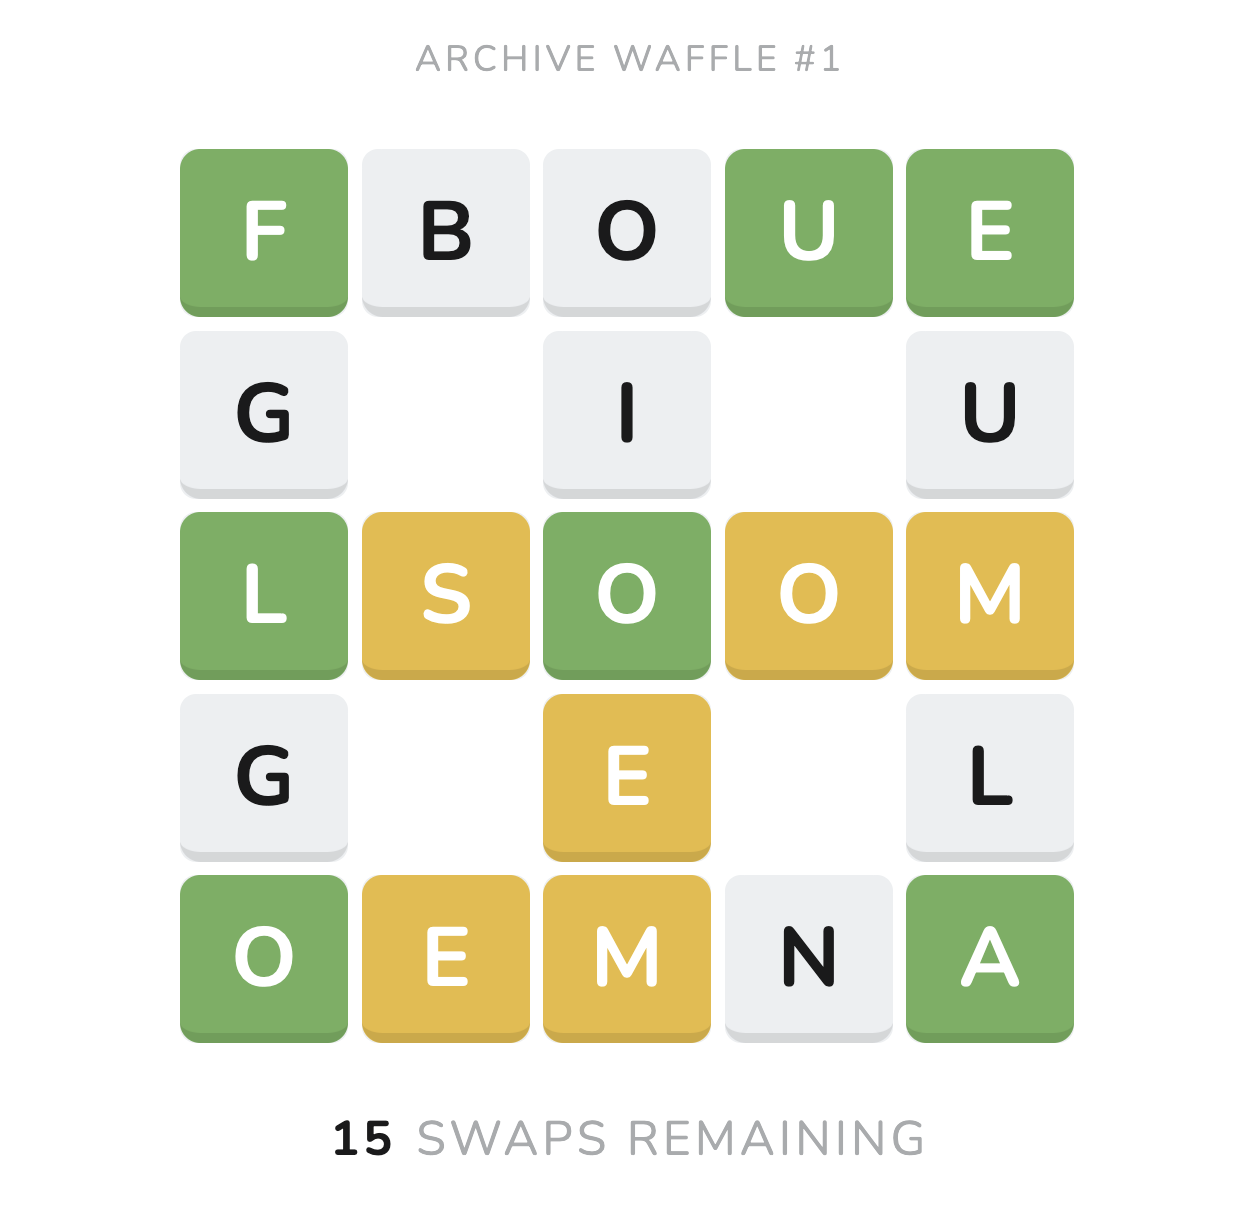
\includegraphics[width=.9\linewidth]{waffle1.png}
\end{center}.  In the original game there are 6 unknown 5 letter
words arranged on a \(5 \times 5\) grid, in the first, third and fifth
rows, and first, third and fifth columns.  Four squares in the grid
are left empty.  The challenge consists in permuting the squares
containing the letters, and then providing clues. 
\subsection{The Challenge}
\label{sec:org94a623c}
The game challenge consists of the following: there is a secret choice
of six words to arrange in the grid.  Then a secret permutation is
chosen by successively choosing 10 pairs of squares and swapping their
contents.  The player gets to choose a pair of squares, and swapping
their contents by dragging one square to the other.  After this move,
the clues (describe below) are updated.  The player gets 15 turns to
restore the grid to its secret state.  The score given is 15 minus the
number of swaps used.
\subsection{The Clues}
\label{sec:org2b517a1}
The permuted squares are given three colors: green, yellow and white.
The color green means that the letter is in a correct position.  The
other colors mean that the letter is in an incorrect position.  Within
each row or column, if all letters with the same value are colored
white, this means that the other positions in the row/column cannot
contain that letter.  In general, the color yellow means that some
other position in the row/column \textbf{will} contain that letter.  Things
get a bit more complicated if there are multiple positions containing
the same letter, some colored yellow, and some colored white.

Here is the more complex rule:

Call a square in the grid \textbf{internal} if it is only contained in one
row or column.  Otherwise call it external.

The rule appears to be that if there are \(a\) positions colored white,
and \(b\) internal positions colored yellow, and \(c\) external positions
colored yellow.  Then at least \(b\) of the remaining squares in that
row/column, not colored green must contain the letter in question, and
not more than \(b + c\) squares may contain the letter in question.
\subsection{Analysis}
\label{sec:org0b2aeb3}
One thing that is \textbf{not} specified on the website is the contents of
the dictionary of allowed five letter words.  I decided to use the
list of official answer for Wordle, which consists of 2309 words.

After seeing the game, and playing it for a number of weeks I wondered
how often the initial set of clues uniquely determine the set of
correct words.  If so, one could then calculate the smallest number of
swaps necessary to restore the grid to its secret state.  In order to
explore this question, I wrote a program using a SAT solver.  I found,
in all cases that I tried, that the initial set of clues uniquely
specified the secret arrangement.  Below I'll describe the encoding
and constraints that I used. 

In analyzing the clues, the first information that they provide is the
multiset of letters in answer.  Since any permutation of the squares
in the grid preserves the multiset, we can add that as a constraint.

Variables: There are two sets of variables.  The first is the \textbf{word
variables} \(w_{\alpha, i}\), where \(\alpha\) ranges over all the words
in the dictionary, and \(i\) ranges over the six rows and columns in the
grid.  This indicate that the word \(\alpha\) is assigned to row/column
\(i\).  The \textbf{square variables} \(s_{q,\ell}\).  This indicates that letter
\(\ell\) is assigned to square \(q\).

The two sets of variables are linked by adding implications
\(w_{\alpha, i} \Rightarrow s_{q,\ell}\) if square \(q\) is contained in
row/column \(i\), colored green, and containing the letter \(\ell\).

We add constraints which ensure that every row/column \(i\) is assigned
a word \(\bigvee_{\alpha} w_{\alpha,i}\), and that no word is used more
than once (this is not specified in the problem description, but it
seems a reasonable assumption): \({\tt Card}(\{w_{\alpha,i}: i\}) \le 1\).

For the clues, the green squares are the most straightforward: we add
a unit clause \(s_{q,\ell}\) to ensure that letter \(\ell\) is assigned to
square \(q\).
\section{A Problem in Computational Group Theory}
\label{sec:org487875f}

To finish up the problem we need to solve the following problem:
determine a permutation of the squares which restores the grid to
contain the secret answer realized as a composition of the smallest
possible number of transposoitions.  Once we have the secret solution
determined, it is easy to determine \textbf{some} permutation \(\pi\) which
does the job.  However, because there are duplicate letters, let
\(G\) be the subgroup of permutations of the squares which leave the
letters invariant.  Then the coset \(G \pi\) is the set of possible
permutations.  We use the following result:

Proposition: Let \(\pi\) be a permutation of \(\{1, \dots, n\}\).  If \(k\)
is the smallest number of transpositions \(\tau_1, \dots, \tau_k\) such
that \(\pi = \tau_1 \cdot \tau_k\), then \(k = n - t\), where \(t\) is the
number of cycles in \(\pi\).

Problem: Let \(G\) be a subgroup of \(S_n\) given by a list of generators
\(g_1, \dots, g_m\), and \(\pi \in S_n\).  Determine an element of \(G \pi\)
with the largest number of cycles.

Question: Can this be done using the Schreier-Sims algorithm?
\section{Sampling Waffle grids}
\label{sec:org0f29621}

If we have a vocabulary list, \(L\), we would like to uniformly sample
all possible \(n \times n\) waffle grids (here \(n\) is odd).  A path to
this goal is via the Metropolis-Hastings algorithm.  The idea of the
MH algorithm is to construct a distribution \(\mathcal{D}\) of all grids
populated by letters, whether valid (i.e. composed of only words in
the vocabulary, with no duplicated words) or not.  We would like there
to be a positive constant \(c > 0\) so that \(\Pr_{\mathcal{D}}(w) = c\)
for each valid grid.  If we can (approximately) sample from
\(\mathcal{D}\) then we can use rejection sampling: keep generating a
sample \(X \sim \mathcal{D}\) until \(X\) is valid.

The Metropolis-Hastings algorithm constructs an ergodic, reversible
Markov chain from an \textbf{energy function} \(E(w) \ge 0\), where \(E(w) = 0\)
if and only if \(w\) is valid.  The Markov chain will thus have a unique
invariant distribution, which will be our sought for distribution
\(\mathcal{D}\).

Let \(\pi(x)\) denote the invariant distribution of the Markov chain and
\(\mu(x,y)\) denote the transition probability of going from state \(x\)
to state \(y\).  Then the reversibility condition is
\(\pi(x)p(x,y) = \pi(y) p(y,x)\).

In the simple chain described in "It's Puzzling", we have
\(p(x,y) = 1/N(x) \min(1, \exp( - \Delta E(x,y)/ T)\) if \(y\) is a
neighbor of \(x\), and \(N(x)\) is the number of neighbors of \(x\), and 0
otherwise.   We set \(p(x,x) = 1 - \sum_{y \sim x} p(x,y)\), where \(y
\sim x\) indicates that \(y\) is a neighbor of \(x\).  Here \(\Delta E(x,y)
= E(y) - E(x)\), where \(E(x) \ge 0\) is an energy function.

We set \(Z = \sum_x \exp(-E(x) / T)\).  We want \(\mu(x) = \exp(-E(x)/T)
/ Z\).  

Suppose that we change the transition probabilities.
\section{Samplers}
\label{sec:orgdebecee}
There's an extensive literature about uniform (or close to uniform)
samplers for SAT.  In particular, Meel, and his collaborators have
also described testers for being close to uniform.  In "Testing of
Horn Samplers", Ansuman Banerjee, Shayak Chakraborty, Sourav
Chakraborty, Kuldeep Meel, Uddalok Sarkar, and Sayantan Sen, describe
a testing procedure for Horn Samplers.  Recall that a \textbf{Horn Clause} is
one in which at most 1 of the literals is positive.  A system of \textbf{renameable
Horn Clauses} is  one in which there is a favored parity for each
literal, and each clause contains at most 1 literal which has the
opposite of the favored parity.

In the SAT formulation for placement of words on a a board, we have
the following sets:
\begin{itemize}
\item \(W\) is the set of words in the vocabulary
\item \(P\) is the set of "places" (rows or columns)
\item \(A\) is the alphabet.
\end{itemize}

We have boolean variables:
\begin{itemize}
\item \(w_{i,j}\): true if and only if the \$i\$-th
\end{itemize}
word is placed on place \(j \in P\)
\begin{itemize}
\item \(s_{\ell,t}\): true if and only if the
\end{itemize}
\$\(\ell\)\$-th letter is placed on square \(t\). Here \(\ell \in A\).

We have the following constraints:

\begin{enumerate}
\item At most one of \(\{w_{i,j}: j \in P\}\) (no repeats).
\item Exactly one of \(\{w_{i,j} : i \in W\}\) (each place gets a word).
\item \(w_{i,j} \Rightarrow s_{\ell,t}\) if square \(t\) is the \$k\$-th square in
place \(j\), and \(\ell\) is the \$k\$-th letter in word \(i\).
\item (optional) Exactly one of \(\{s_{\ell,t}: \ell \in A\}\) for all \(t\).
\end{enumerate}
(this can be relaxed to at most one, since (2) and (3) imply that at
least one is true).
\section{More about swaps}
\label{sec:orgaf46560}
To generate the secret permutation, it is disallowed to swap two
locations that contain the same letter.  It is not clear what method
is used by Robinson (the puzzle constructor).  Empirically, all of the
permutations really do require 10 swaps.  If the rule of disallowing
swapping two locations with the same letter was not enforced one could
use the characterization of the minimum distance on the Cayley graph
where the generators are all transpositions, of being the degree of
the permutation group minus the number of cycles in the permutation.
Instead, if the positions are the set \(P\) and the letters are the set
\(L\), we are interested in a subgroup of the wreath product \(S(P) \wr
S(L)\).  This group is generated by transpositions of the form \(((p,c),
(p',c'))\), where \(p \ne p, c \ne c'\).  I believe that with this
generating set, this is a Coxeter group, since for \(x,y,z\) distinct we
have \((x,y)(x,z) = (x,y,z)\)  of order 3, these relations completely
characterize the group.  Another clue to his generation method is that
all of the even numbered puzzles have left right symmetry in the
colors of the permuted grid.
\end{document}
